\section{Further extensions}
\label{sec:futurework}

This section details further extensions on improving other aspects of the 
visualization system. To improve the methods discussed in this paper, see the 
final ``extensions'' section in the Chapter~\ref{ch:al} for active learning and 
Chapter~\ref{ch:gc} for graph comparison.

\subsection{Estimator selection}
\label{sec:futurework:estimatorselection}

Estimator selection involves actively fitting the best model as opposed to
``checking'' a numerical model that’s been given. For instance, rather than 
requiring a numerical model in order to check for graph distance 
(Chapter~\ref{ch:gc}), the VS would select a numerical model without requiring 
the analyst to fit one beforehand. This problem is more difficult
to define, and the value that the visualization system adds is not as concrete.

\subsection{Outlier removal}
\label{sec:futurework:outlier}

Outliers are unavoidable in raw data and can skew results quite a bit. This can 
be seen in the analysis of Dataset 2 in Table~\ref{tab:intro:me} and 
Figure~\ref{fig:intro:meplot}. 

((When can the system remove outliers? What criteria should it use? ))

\subsection{Graphical models and improved stock selection}
\label{sec:futurework:graphicalmodel}

A single correlation (discussed in Section~\ref{sec:intro:correlation}) can be 
thought of as a regression of the response variable
against only one observed variable; it is a ``local'' property because it
compares the behavior of only two random variables. On the other hand, a single
link in a graphical model can be thought of as a regression of the response
variable against all variables in the space. The general idea is that a 
graphical model has a ``global'' property because it takes all
of the other variables into account. Although it may seem simple to numerically
quantify the dependencies with correlation as conditional dependencies are less
intuitive to compute, correlations tend to fall short of the desired result due
to the property of transitivity.

Transitivity states that if $X$ is correlated to $Y$, and $Y$ to $Z$,
then $X$ is also correlated to $Z$. Although correlation is not always
transitive, situations where the correlation is close to 1 or 0, then the
transitivity of correlation can be recovered and observed in the relevant
data~\cite{tao2014}. Let us assume that the universe consists of Apple, Google, 
and Silicone (a manufacturer providing chips to both Apple and Google) stock. 
Suppose an analyst wants to model Google stock. 
Apple stock moves with Silicone stock as they
depend on them for their chips. Similarly, Google stock (unbeknownst to the
analyst) also moves with Silicone stock but not with Apple stock. The
correlation between observed prices of Google and Apple stock will clearly and
erroneously be positive without considering the way the stocks are connected to
the other observed variable (Silicone stock). Given that correlation tends to be
transitive, a correlation graph can have too many edges. This goes against the
concept of ``sparsity'' (Section~\ref{sec:intro:finance}) by cluttering the 
resulting space of observation
variables that explain the response variable for the user, leaving the
analyst with an uninformative and unaccountable numerical solution.

Graphical models alleviate some of the problems associated with correlation
graphs, but they have their own set of problems, as well. Let $G=(V,E)$ be an
undirected graph with vertices $V_1,...,V_d$ (a
$d$-dimensional distribution) and edges $E_{i,j}\in\{0,1\}$. We set $E_{i,j}=1$
when there is an edge between $V_i$ and $V_j$, and 0 otherwise. Do not draw an
edge between $V_i$ and $V_j$ iff $V_i \perp V_j$ given $V_k$ where
$k\in\{1,...,d\}$ \textbackslash $\{i,j\}$. In other words, do not draw an edge
if
$$\text{P}(V_i,V_j|V_k)=\text{P}(V_i|V_k)\text{P}(V_j|V_k)$$

This result is known as a graphical model. The drawback is the difficulty in
empirically computing conditional distributions and the problems associated with
fitting distributions to real data. While there are simplifications that can be
made for plotting, the solution is not always so clear. 
However, the conditional independence of
graphical models is more of a global property than correlation is because, for
every pair of variables, it conditions on all the remaining variables. Returning
to the universe of Google, Apple, and Silicone stocks, conditioning Google on
Silicone and Apple on Silicone makes the relationship between the two clearly
uncorrelated. Thus, although conditional independence tends to be more difficult
to determine, it will tend to give a sparser network that is more interpretable
for the analyst.

Correlation graphs and graphical models 
each have their own niche to fill, though a graphical model rebalancing has 
been shown to strongly outperform traditional portfolio management 
methods~\cite{liuh2016}. It is important, therefore, for the VS to 
support both models. The system would need to be modified to allow for plotting 
$V_i$ against $V_j$ conditional on $V_k$ for all $k\in\{1,...,d\} \backslash 
\{i,j\}$. One method to consider would be to control for the behavior of all 
the other explanatory variables while making this scatter plot, similar to 
regression.

\subsection{Ordering of queried plots}
\label{sec:futurework:ordering}

As people interact with graphs, they maintain a ``mental map'' of the 
graph; when users label a new graph, they remember the previous plots that they
have labeled~\cite{federico2016}. The importance of the mental map depends on
various factors such as the user preferences and tasks that they must
complete~\cite{federico2016}. Suppose that several active learning queries 
(scatter plots) are selected at once. Given a gradation of graphs (showing 
graphs that are most alike one after the other), users are less able to 
distinguish between differences than if they are shown graphs from different 
ends of the spectrum at different times~\cite{federico2016}. To put it 
concisely, the scatter plot display itself (discussed in 
Section~\ref{sec:visualizer:scatterplot:goodplot}) is not the only thing that 
matters. The ordering of the display matters, as well, and it is best to show 
the plots in an order that allows users to distinguish the differences among 
graphs that they have already seen. By improving their understanding of the 
plots, careful display ordering advances the accuracy of user responses. User 
responses can be thought of as observations of the user’s true preferences, and 
the ordering of plots as a way to fine-tune the precision of the classifier. 

\subsection{Line-up tests}
\label{sec:futurework:lineup}

One of the pitfalls of data visualization is ``apophenia,'' a phenomenon where
the user sees patterns in random noise. Part of the reason for this is due to
the vagueness of defining ``independence'' on a non-uniform domain and range
(Section~\ref{sec:visualizer:scatterplot:goodplot}). Wickham \textit{et al.} 
propose a line-up protocol that is similar to the Rorscach test where subjects 
are asked to interpret abstract blots of ink~\cite{wickham2010}. 
In the line-up test,
users are asked to identify the real data from a set of n plots where $n – 1$
plots are synthetically generated (Figure\ref{fig:visualizer:lineup}). 
Identification of the raw data against the synthetic data is then an indicator 
that the current fitted model is a poor fit of the user's preferences.
In the context of the classification problem, the learner may generatae
four ``uninteresting'' plots (following the proposed decision tree) with one
``interesting'' plot and asks the user if he/she can identify the interesting
plot. If the user is able to consistently identify the interesting plot, it is
an indication that the current decision tree is a close fit of the user’s
preferences.

\begin{figure}[H]
	\begin{center}
		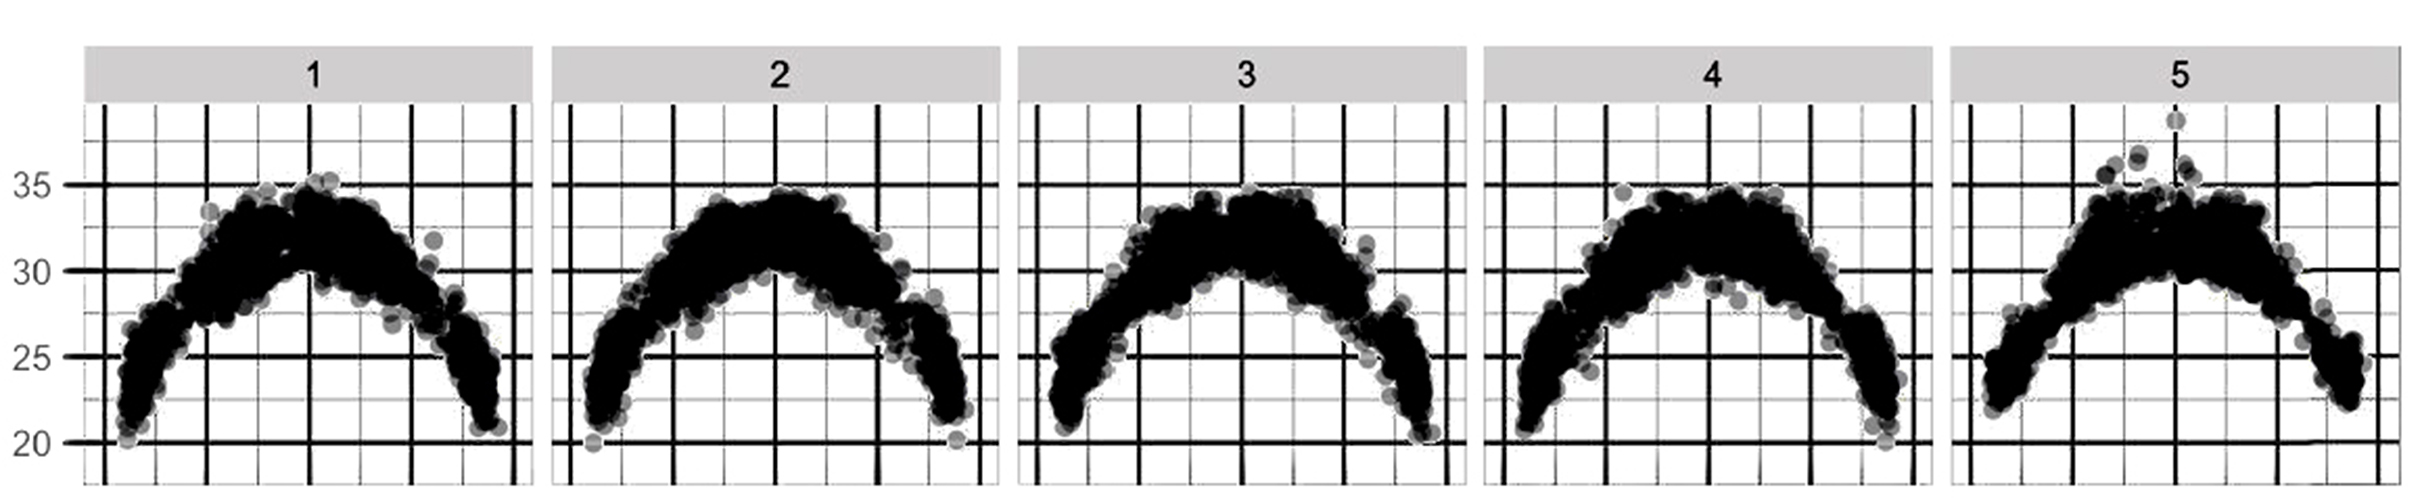
\includegraphics[width=1\linewidth]{ch-conclusion/figures/lineup}
		\caption[A line-up test for $n = 5$. ]{A line-up test for $n = 5$.
			Consistently identifying the raw data against the synthetic data 
			indicates that
			the fitted model may not be good enough. Figure from Wickham 
			\textit{et al.}~\cite{wickham2010}}
		\label{fig:visualizer:lineup}
	\end{center}
\end{figure}

\subsection{Edge-weighted graphs}
\label{sec:futurework:edgeweighted}

Edge-weighted graphs also stray from the black and white classification of 
correlation graphs (Section~\ref{sec:intro:correlation}) and graphical models 
(Section~\ref{sec:futurework:graphicalmodel}) which have been discussed 
earlier. In an edge-weighted graph, edges can be weighted depending
on the type of conditional dependence or correlation. Negative or positive 
values are assigned 1 or -1, respectively. A value of 0 (no edge) still implies 
conditional independence or uncorrelated variables. This problem is more 
difficult as the number of classification labels changes from two to three, and 
the graph has become more information but complex. 
Active learning methods may need to be more generalized as in the case of 
uncertainty sampling (Section~\ref{sec:al:methods:uncertainty}). 

\subsection{Rejection classification}
\label{sec:futurework:rejection}

So far, classification has been discussed in terms of black and white, 
interesting versus non-interesting. While interacting with the data visually, 
the user's concept of what's interesting in the specific dataset may evolve 
over time; at the beginning, they have no idea what the data looks like and 
where to set the bar for their own standards of dependence. There are several 
ways to take this into consideration. 

\tablespacing
\begin{itemize}
	\item The visualization system could assign a weight to the analyst's 
	responses by trial number where the last few plots are more valuable than 
	the first few. However, this may destabilize cases where the user's 
	preferences don’t end up changing.
	\item The system can include an alternative option that allows the user to 
	refuse to label a plot when it's too close to their decision boundary. This 
	is welcome for the user who is not forced into making a decision he/she is 
	uncertain about, but it is problematic for the learner as it causes the 
	hypothesis space to remain unchanged rather than shrink. The point of the 
	active learning in stage 1 (Section~\ref{sec:visualizer:al}, 
	Chapter~\ref{ch:al}) is to have the oracle provide labels in order to 
	better understand user preferences. By allowing for this option, the active
	learner may run for too long and/or return a poorly-defined tree. 
	\item The system can contain a third option that permits the user to 
	``recycle'' the plot. This allows to user to return to the plot later after 
	learning more about what the data looks like and understanding his/her own 
	preferences better, and it ensures that the active learner will eventually 
	receive data on the ambiguous plots that it has queried. The main concern 
	is that this could potentially de-balance an ordering procedure 
	(Section~\ref{sec:futurework:ordering}), but the system can strategically 
	insert the recycled plot between two plots it differs from with the 
	constraint that the insertion location is after the current plot.
\end{itemize}
\bodyspacing
